\chapter{The First Paper/Chapter}

\section{Introduction}

We begin with the most important question in political science. \lipsum[1]

\section{Literature}

The literature on this question begins with  \citet{tocqueville1838} and \citet{wilson1885}. There is also some more literature \citep{downs1957,baron1989,cox1993,krehbiel1998}. \lipsum[2]

\section{Some Results}

See Table~\ref{tab:example1} and Figure~\ref{fig:example2}. \lipsum[3] 

\begin{table}[htbp]
\caption{Captions for Tables Go \textbf{ABOVE} the Table}
\label{tab:fjc_summary}
\begin{center}
\begin{tabular}{llrrrrrrr}
\toprule
& First & Total & Appts. & Appts. & Avg. & Original & Current & Currently\\
Court & Year & Appts. & Per Year & Per Pres. & Tenure & Seats & Seats & Serving\\
\midrule
USSC & 1789 & 117 & 0.53 & 2.67 & 16.06 & 6 & 9 & 9 \\ 
USCA & 1891 & 729 & 6.18 & 26.42 & 13.87 & 18 & 179 & 164 \\ 
USDC & 1789 & 2826 & 12.85 & 61.70 & 14.56 & 13 & 673 & 597 \\ 
\bottomrule
\end{tabular}
\end{center}
\end{table} 

\lipsum[4]

\begin{figure}[htbp]
   \centering
   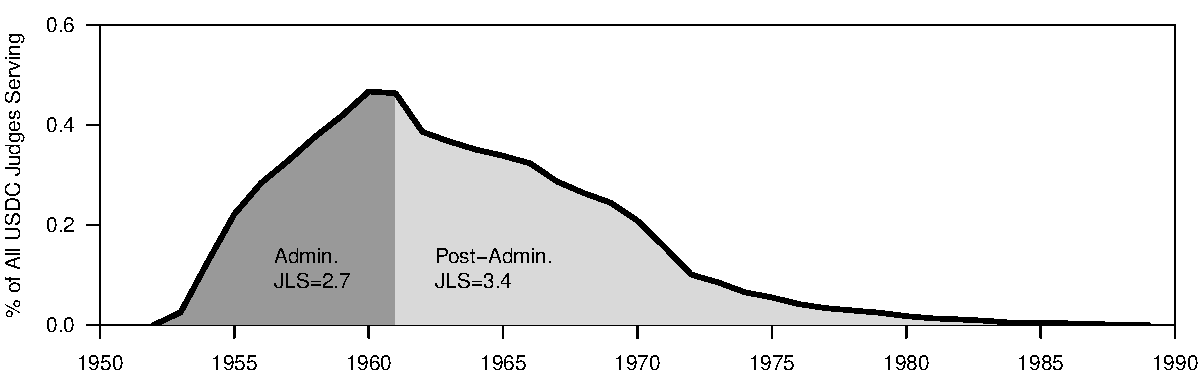
\includegraphics[width=\textwidth]{figures/example_figure.pdf}
   
\caption{Captions for Figures Go \textbf{BELOW} the Figure}
\label{fig:example2} % Label must go below the caption
\end{figure}

\lipsum[5]

\section{Conclusion}
\lipsum[6-7] 